\documentclass[12pt]{article}
\usepackage[english]{babel}
\usepackage[utf8]{inputenc}

%% Pointer to 'default' preamble
% pacakages and definitions

\usepackage{geometry}
\geometry{
	letterpaper, 
	portrait, 
	top=.75in,
	left=.8in,
	right=.75in,
	bottom=.5in		} 	% Page Margins
	
%% additional packages for nice things
\usepackage{amsmath} 	% for most math
\usepackage{commath} 	% for abs
\usepackage{lastpage}	% for page count
\usepackage{amssymb} 	% for therefore
\usepackage{graphicx} 	% for image handling
\usepackage{wrapfig} 	% wrap figures
\usepackage[none]{hyphenat} % for no hyphenations
\usepackage{array} 		% for >{} column characterisctis
\usepackage{physics} 	% for easier derivative \dv....
\usepackage{tikz} 		% for graphic@!
\usepackage{circuitikz} % for circuits!
\usetikzlibrary{arrows.meta} % for loads
\usepackage[thicklines]{cancel}	% for cancels
\usepackage{xcolor}		% for color cancels
\usepackage[per-mode=fraction]{siunitx} % for si units and num
\sisetup{group-separator = {,}, group-minimum-digits = 3} % additional si unit table functionality

\usepackage{fancyhdr} 	% for header
\usepackage{comment}	% for ability to comment out large sections
\usepackage{multicol}	% for multiple columns using multicols
\usepackage[framed,numbered]{matlab-prettifier} % matlab sytle listing
\usepackage{marvosym} 	% for boltsymbol lightning
\usepackage{pdflscape} 	% for various landscape pages in portrait docs.
%\usepackage{float}
\usepackage{fancyvrb}	% for Verbatim (a tab respecting verbatim)
\usepackage{enumitem}	% for [resume] functionality of enumerate
\usepackage{spreadtab} 	% for using formulas in tables}
\usepackage{numprint}	% for number format in spread tab
\usepackage{subcaption} % for subfigures with captions
\usepackage[normalem]{ulem} % for strike through sout

% for row colors in tables....
\usepackage{color, colortbl}
\definecolor{G1}{gray}{0.9}
\definecolor{G2}{rgb}{1,0.88,1}%{gray}{0.6}
\definecolor{G3}{rgb}{0.88,1,1}

% For table formatting
\usepackage{booktabs}
\renewcommand{\arraystretch}{1.2}
\usepackage{floatrow}
\floatsetup[table]{capposition=top} % put table captions on top of tables

% Caption formating footnotesize ~ 10 pt in a 12 pt document
\usepackage[font={small}]{caption}

%% package config 
\sisetup{output-exponent-marker=\ensuremath{\mathrm{E}}} % for engineer E
\renewcommand{\CancelColor}{\color{red}}	% for color cancels
\lstset{aboveskip=2pt,belowskip=2pt} % for more compact table
%\arraycolsep=1.4pt\def
\setlength{\parindent}{0cm} % Remove indentation from paragraphs
\setlength{\columnsep}{0.5cm}
\lstset{
	style      = Matlab-editor,
	basicstyle = \ttfamily\footnotesize, % if you want to use Courier - not really used?
}
\renewcommand*{\pd}[3][]{\ensuremath{\dfrac{\partial^{#1} #2}{\partial #3}}} % for larger pd fracs
\renewcommand{\real}[1]{\mathbb{R}\left\{ #1 \right\}}	% for REAL symbol
\newcommand{\imag}[1]{\mathbb{I}\left\{ #1 \right\}}	% for IMAG symbol
\definecolor{m}{rgb}{1,0,1}	% for MATLAB matching magenta
	
%% custom macros
\newcommand\numberthis{\addtocounter{equation}{1}\tag{\theequation}} % for simple \numberthis command

\newcommand{\equal}{=} % so circuitikz can have an = in the labels
\newcolumntype{L}[1]{>{\raggedright\let\newline\\\arraybackslash\hspace{0pt}}m{#1}}
\newcolumntype{C}[1]{>{\centering\let\newline\\\arraybackslash\hspace{0pt}}m{#1}}
\newcolumntype{R}[1]{>{\raggedleft\let\newline\\\arraybackslash\hspace{0pt}}m{#1}}

%% Header
\pagestyle{fancy} % for header stuffs
\fancyhf{}
% spacing
\headheight 29 pt
\headsep 6 pt

%% Header
\rhead{Thad Haines \\ Page \thepage\ of \pageref{LastPage}}
\chead{Variable time step ODE45\\ Compared to fixed step lsim using a state space PSS model}
\lhead{Research \\ 6/30/20}

\usepackage{minted}
\usepackage{setspace}
\usepackage{lscape}
\usepackage{multicol}
\begin{document}
\onehalfspacing
\paragraph{Step Results of a 3rd Order State Space System} \ \\
A fixed time step of 1/4 cycle ($\approx$4.2 seconds) using \verb|lsim| was compared to a variable time step \verb|ode45| solution.
The default ODE tolerance settings were altered to produce an acceptable match in output (code line 23).

Data output plots appear the same upon inspection.
The variable time step method requires fewer steps ($\approx 5.5$x less in this example) for very similar output.
Time step size seems to oscillate around 0.026 seconds post-perturbance but is as large as 0.13 seconds before the step is executed.

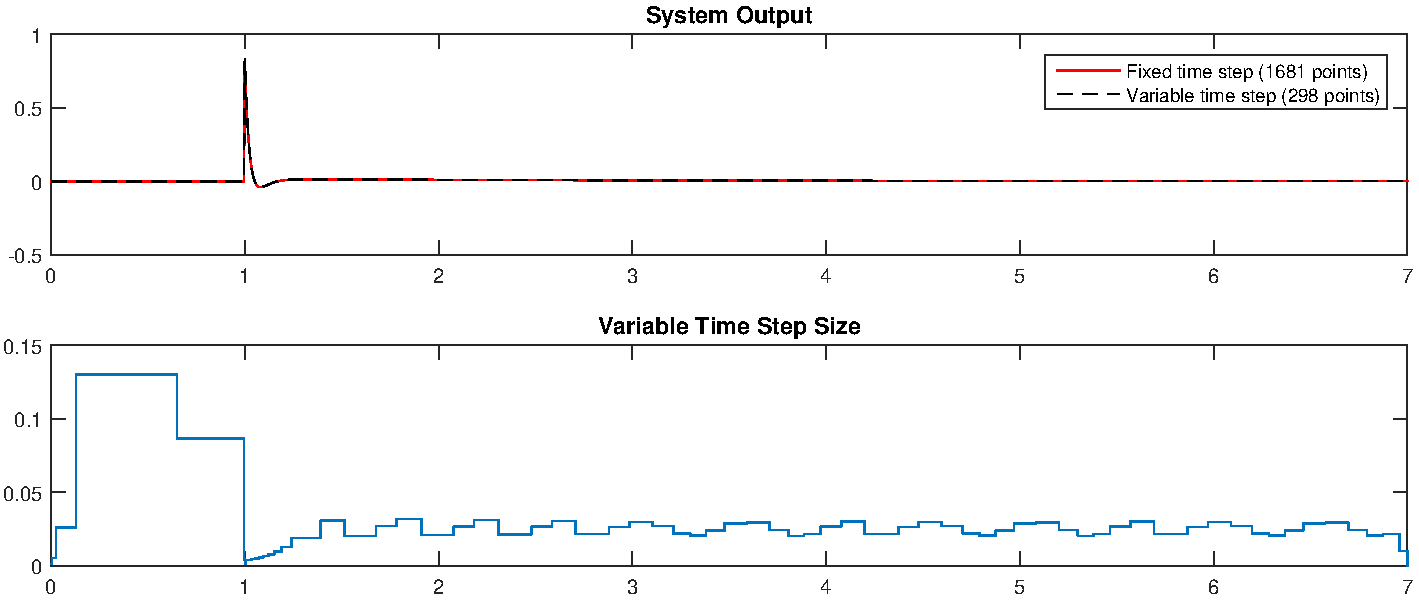
\includegraphics[width=\linewidth]{step}

A detail view of the output shows minor oscillations of the variable time step results around the fixed step results and the time step increasing and deceasing accordingly.

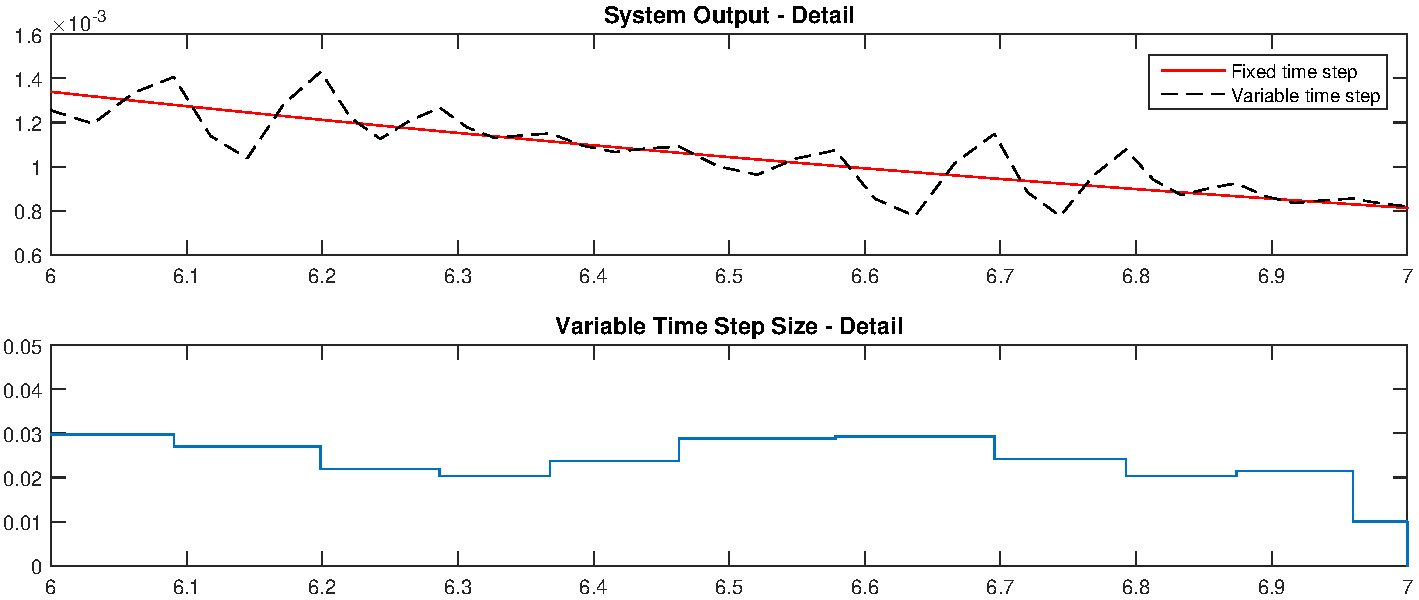
\includegraphics[width=\linewidth]{stepDetail}

\pagebreak
Running the simulation out to 60 seconds shows that this \emph{time step oscillation} occurs continuously after an event.
The large decease in time step size near the end of a calculated time interval appears to be a common \verb|ode45| trait.

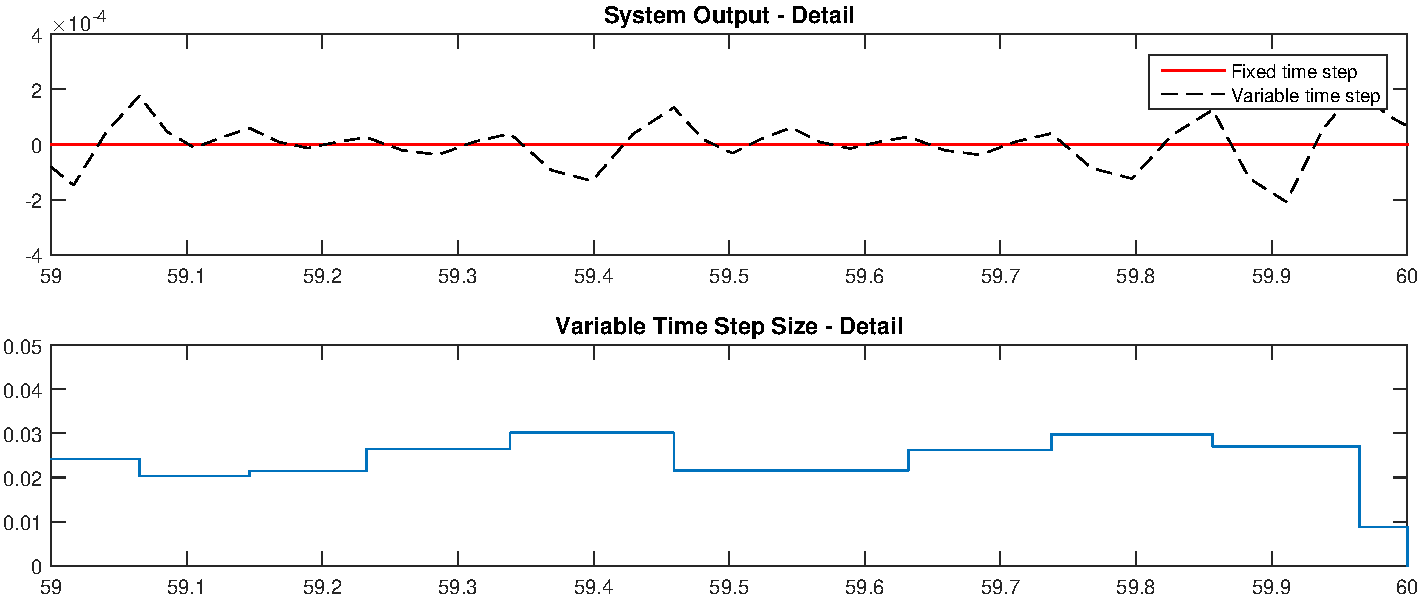
\includegraphics[width=\linewidth]{stepDetail2}


\paragraph{MATLAB Code} \ \\
The \verb|ode45| function requires a passed in function that uses \verb|t| and returns derivatives.
A simple \verb|getXdot| function was written that performs such an action.
Note that the time variable \verb|t| is not used and most variables are global.
This was done done to mimic PST methods.
\begin{minted}[
		frame=lines,
		framesep=2mm,
		baselinestretch=1.2,
		bgcolor=gray!13,
		fontsize=\footnotesize,
		%linenos,
		breaklines
		]{MATLAB}
function [ xdot ] = getXdot( t, x)
%getXdot return xdot from statespace for ODE45 use
%   t = filler variable
%   A = A matrix from system
%   x = initial state vector
%   B = B matrix from system
%   U = Input to system
global A B U
    xdot = A*x + B*U;
end		
\end{minted}
A PSS model from the miniWECC case was used as the system to test.
Manipulation of \verb|ode45| output is required for correct state operation and model output handling (lines 36 and 41).

\verb|ode45| has a 'OutputFcn' option that may be useful in indexing, time advancement, required state/output handling, and/or network solution calls.
Other \verb|ode45| options exist that may also be useful in future development.

\pagebreak
\begin{minted}[
		frame=lines,
		framesep=2mm,
		baselinestretch=1.2,
		bgcolor=gray!13,
		fontsize=\footnotesize,
		linenos,
		breaklines
		]{MATLAB}
%% test to use ode solver to step PST-esq model
close all;clear;format compact;clc

%% pss model definition (miniWECC)
%           1   2   3   4       5   6   7       8       9       10
pss_con = [ 1  	1   20  2     0.25 0.04 0.2   0.03      1.0     -1.0];

%% MATLAB model
tend = 60;
block1 = tf([pss_con(3)*pss_con(4), 0],[pss_con(4), 1]);
block2 = tf([pss_con(5), 1],[pss_con(6), 1]);
block3 = tf([pss_con(7), 1],[pss_con(8), 1]);

G= block1*block2*block3;
tL = 0:1/60/4:tend; % quarter cycle steps
modSig = zeros(size(tL,1),1);
modSig(tL>=1) = .001; % very small input to avoid limiter
yL = lsim(G,modSig,tL);

%% ODE45 attempt with statespace
% Configure ODE settings
%options = odeset('RelTol',1e-3,'AbsTol',1e-6); % default settings
options = odeset('RelTol',1e-5,'AbsTol',1e-8,'InitialStep', 1/60/4, 'MaxStep',20);

% manipulate test sytem to statespace
[num,den] = tfdata(G);
global A B U
[A,B,C,D] = tf2ss(num{1},den{1});
% initial conditions
x = zeros(size(A,1),1);
y0 = x;
U = 0;

% Pre-perturbance
[t1,y1] = ode45(@getXdot, [0,1-1/60/4],y0, options);
yOut1 = C*y1'+D*U;

% Step input
U = modSig(end);
[t2,y2] = ode45(@getXdot, [1,tend],y1(end,:)', options); 
yOut2 = C*y2'+D*U;

% combining output
tCombined = [t1;t2];
yCombined = [yOut1, yOut2];		
\end{minted}



\end{document}
